\documentclass[../../doc.tex]{subfiles}
\graphicspath{{\subfix{../../img}}}
\begin{document}
    \subsection{Целевое положение схвата}

    В данном разделе мы приведем примеры работы алгоритма для классических задач биологического движения.
    \begin{remark}
        В каждом из примеров, для избежания проворачивания сочленений, в интегральную часть функционала качества дополнительно добавлена поправка
        $$
            10^{-5}\cdot \left\langle x^k, \hat Q x^k \right\rangle.
        $$
    \end{remark}

    Пусть целью нашего движения является достижение схватом заранее определенного положения $e^{\textnormal{final}} \in \mathcal{B}_{0}\left(\sum_{i=1}^{3}l_i\right)$ с заданной скоростью $e^{\textnormal{final}}$.
    Таким образом получаем следующие компоненты функционала качества:
    \begin{equation}
        q^{\textnormal{final}}(x) = \left\| e^3(x) -  e^{\textnormal{final}}\right\|^2
    \end{equation} 

    Аналитически найдем $x^{\textnormal{final}}$, требующийся для построения начального референсного управления из следующих соотношений:
    \begin{equation*}
        \textnormal{tg}\,\theta_3
        =
        \begin{cases}
            \frac{e_2^{\textnormal{final}}}{e_1^{\textnormal{final}}}, & \mbox{при } e_1^{\textnormal{final}} \neq 0,
            \\
            0, & \mbox{иначе}.
        \end{cases}  
    \end{equation*}
    \begin{equation*}
        \begin{cases}
            l_1 \cos \theta_1 + l_2 \cos \theta_2 = e_1^{\textnormal{final}} - l_3 \cos \theta_3,
            \\
            l_1 \sin \theta_1 + l_2 \sin \theta_2 = e_2^{\textnormal{final}} - l_3 \sin \theta_3.
        \end{cases}
    \end{equation*}
    Данная система имеет два решения на рассматриваемом интервале $\theta_1, \theta_2 \in [ -\pi, \pi ]$, которые соответствуют возможному положению руки.
    В работе строились начальные траектории для обоих вариантов, затем для итеративного алгоритма выбиралась траектория с наименьшем значением функционала качества.

    Для скорости минимизации по скорости фиксируем $\dot \theta_1 = 0$, а оставшиеся компоненты так же получаем из соотношений:
    \begin{equation*}
        \begin{cases}
            - l_2 \sin \theta_2 \dot \theta_2 - l_3 \sin \theta_3 \dot \theta_3 = \dot e_1^{\textnormal{final}},
            \\
            \hphantom{-} l_2 \cos \theta_2 \dot \theta_2 + l_3 \cos \theta_3 \dot \theta_3 = \dot e_2^{\textnormal{final}},
        \end{cases}
    \end{equation*}

    \begin{figure}[h]
        \begin{center}
            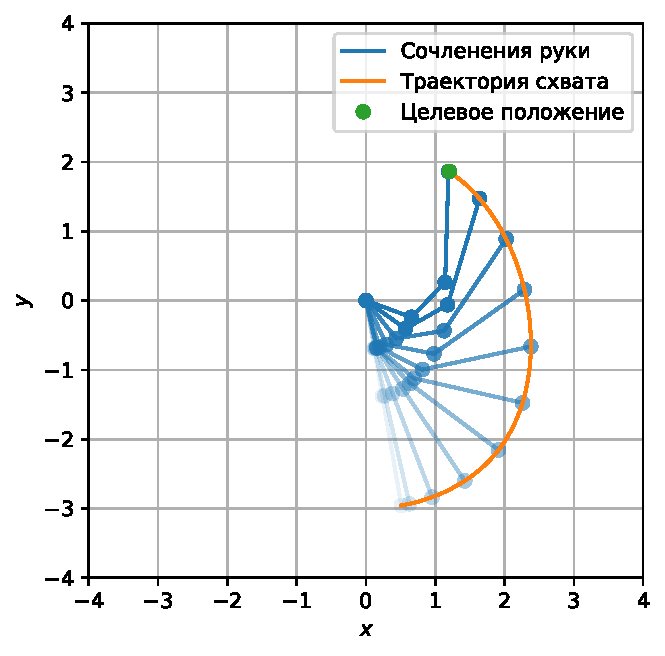
\includegraphics[width=0.49\textwidth]{examples/reaching_pendulum}
            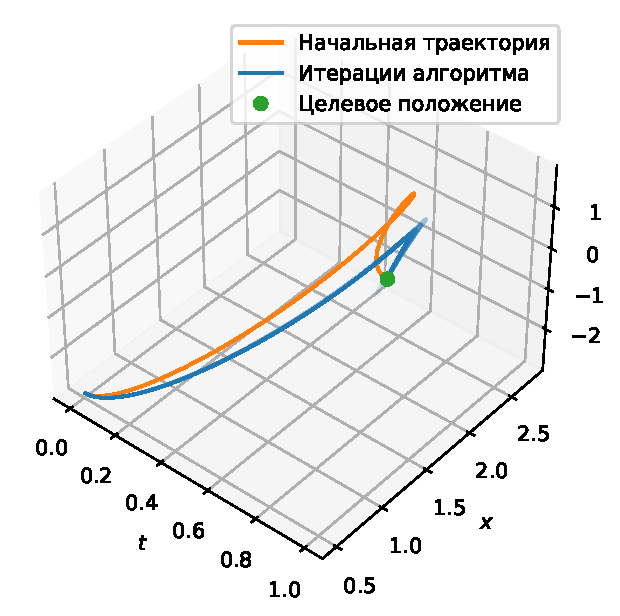
\includegraphics[width=0.49\textwidth]{examples/reaching_endpoint}
        \end{center}
        \caption{Reaching Task}
    \end{figure}

    \begin{figure}[h]
        \begin{center}
            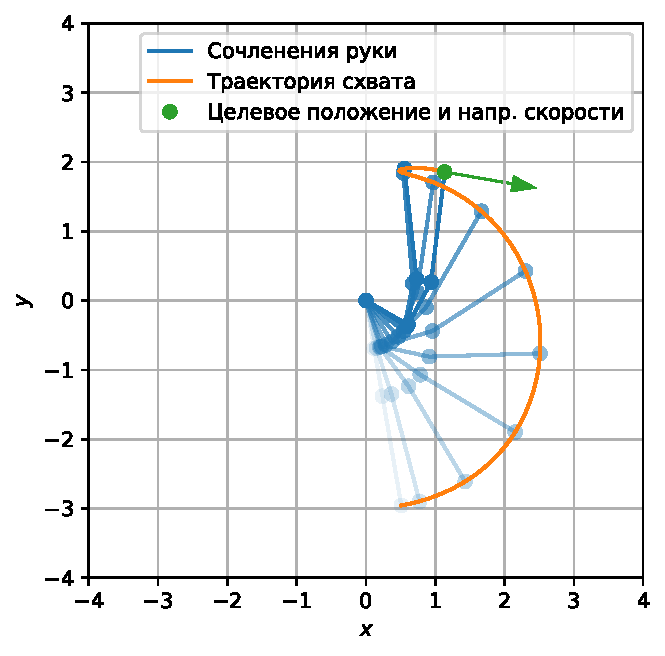
\includegraphics[width=0.49\textwidth]{examples/reaching_speed_pendulum}
            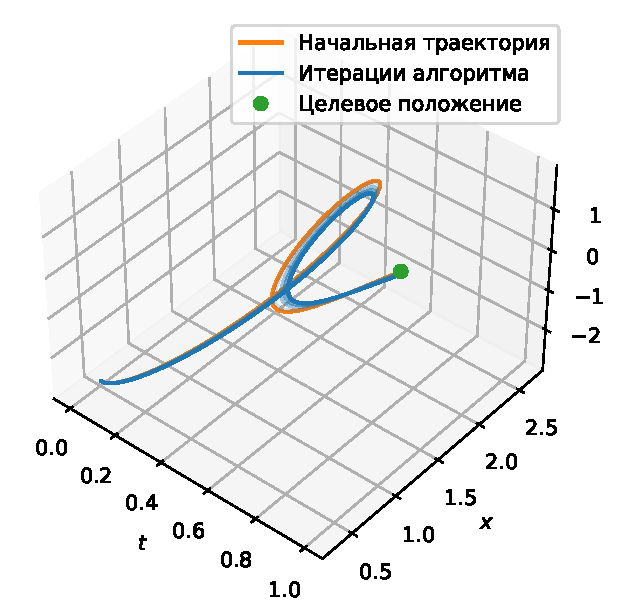
\includegraphics[width=0.49\textwidth]{examples/reaching_speed_endpoint}
        \end{center}
        \caption{Reaching Speed Task}
    \end{figure}

    \ifSubfilesClassLoaded{
        \nocite{*}
        \clearpage
        \bibliographystyle{plain}
        \bibliography{../../refs}
    }{}
\end{document}